%%%%%%%%%%%%%%%%%%%%%%%%%%%%%%%%
% Compile with
% pdflatex --shell-escape -synctex=1 -interaction=nonstopmode meshNormal.tex
% to convert it to png use:
% convert -density 300 -transparent white meshNormal.pdf meshNormal.png
%%%%%%%%%%%%%%%%%%%%%%%%%%%%%%%%

\documentclass{standalone}

\usepackage[utf8]{inputenc}
\usepackage{tkz-fct}
\renewcommand{\familydefault}{\sfdefault}
\usepackage[scaled=1]{helvet}
\usepackage[helvet]{sfmath}
\everymath={\sf}
\usetikzlibrary{calc,arrows,intersections,angles,quotes,patterns}

\definecolor{AFLight}{HTML}{5CE0E6}
\definecolor{AFMiddle}{HTML}{51ADE5}
\definecolor{AFDark}{HTML}{0E4160}

\begin{document}

\tikzset{
   every node/.style={scale=1.3},
   >=stealth
}

\begin{tikzpicture}[
    scale=3
 ]
\def\xMin{0}
\def\xMinSec{1}
\def\yMin{0}
\def\yMinSec{1}
\def\xMax{1}
\def\yMax{1}

\def\xxMin{0.5}
\def\xxMinSec{1.5}
\def\yyMin{0.5}
\def\yyMinSec{1.5}
\def\xxMax{1.5}
\def\yyMax{1.5}
    \foreach \i in {\xMin,\xMinSec,...,\xMax} {
        \draw [dotted, gray] (\i,\yMin-0.5) -- (\i,\yMax+0.5);
    }
    \foreach \i in {\yMin,\yMinSec,...,\yMax} {
        \draw [dotted, gray] (\xMin-0.5,\i) -- (\xMax+0.5,\i);
        \foreach \j in {\xMin,\xMinSec,...,\xMax} {
            \draw [color=AFMiddle] plot [only marks, mark size=1, mark=square*] coordinates {(\j,\i)};
        }
    }

    \foreach \i in {\yyMin} {
        \foreach \j in {\xxMin} {
            \draw [color=AFLight] plot [only marks, mark size=1, mark=*] coordinates {(\j,\i)};
        }

    }


\draw[->, thick, AFDark] (0,0) -- (1,1);
\draw[->, thick, AFDark] (0,1) -- (1,0);


\end{tikzpicture}
\begin{tikzpicture}[
    scale=3
 ]
\def\xMin{0}
\def\xMinSec{1}
\def\yMin{0}
\def\yMinSec{1}
\def\xMax{2}
\def\yMax{2}

\def\xxMin{0.5}
\def\xxMinSec{1.5}
\def\yyMin{0.5}
\def\yyMinSec{1.5}
\def\xxMax{1.5}
\def\yyMax{1.5}
    \foreach \i in {\xMin,\xMinSec,...,\xMax} {
        \draw [dotted, gray] (\i,\yMin-0.5) -- (\i,\yMax+0.5);
    }
    \foreach \i in {\yMin,\yMinSec,...,\yMax} {
        \draw [dotted, gray] (\xMin-0.5,\i) -- (\xMax+0.5,\i);
        \foreach \j in {\xMin,\xMinSec,...,\xMax} {
            \draw [color=AFMiddle] plot [only marks, mark size=1, mark=square*] coordinates {(\j,\i)};
        }
    }

    \foreach \i in {\yyMin,\yyMinSec,...,\yyMax} {
        \foreach \j in {\xxMin,\xxMinSec,...,\xxMax} {
            \draw [color=AFLight] plot [only marks, mark size=1, mark=*] coordinates {(\j,\i)};
        }

    }

\draw (0.75,1.25) node[color=AFDark] {$1$};
\draw (1.25,1.25) node[color=AFDark] {$2$};
\draw (1.25,0.75) node[color=AFDark] {$3$};
\draw (0.75,0.75) node[color=AFDark] {$4$};

\draw[->, thick, AFDark] (1,1) -- (1,2);
\draw[->, thick, AFDark] (1,1) -- (2,1);
\draw [dotted, AFDark, thick] (1,2) -- (2,1);
\draw[->, thick, AFDark] (1,1) -- (1,0);
\draw [dotted, AFDark, thick] (2,1) -- (1,0);
\draw[->, thick, AFDark] (1,1) -- (0,1);
\draw [dotted, AFDark, thick] (1,0) -- (0,1);
\draw [dotted, AFDark, thick] (0,1) -- (1,2);


\end{tikzpicture}
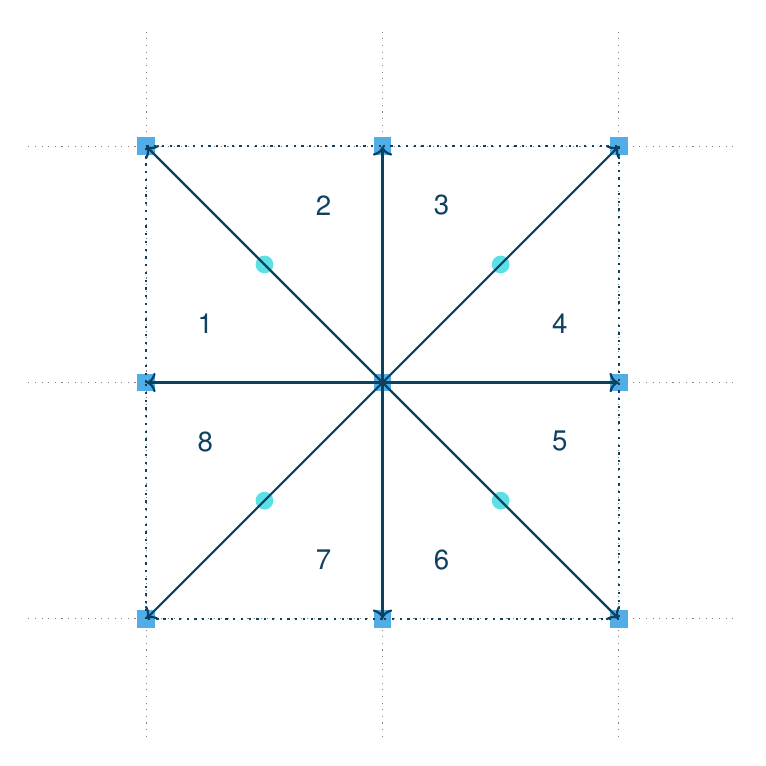
\begin{tikzpicture}[
    scale=3
 ]
 \def\xMin{0}
\def\xMinSec{1}
\def\yMin{0}
\def\yMinSec{1}
\def\xMax{2}
\def\yMax{2}

\def\xxMin{0.5}
\def\xxMinSec{1.5}
\def\yyMin{0.5}
\def\yyMinSec{1.5}
\def\xxMax{1.5}
\def\yyMax{1.5}
    \foreach \i in {\xMin,\xMinSec,...,\xMax} {
        \draw [dotted, gray] (\i,\yMin-0.5) -- (\i,\yMax+0.5);
    }
    \foreach \i in {\yMin,\yMinSec,...,\yMax} {
        \draw [dotted, gray] (\xMin-0.5,\i) -- (\xMax+0.5,\i);
        \foreach \j in {\xMin,\xMinSec,...,\xMax} {
            \draw [color=AFMiddle] plot [only marks, mark size=1, mark=square*] coordinates {(\j,\i)};
        }
    }

    \foreach \i in {\yyMin,\yyMinSec,...,\yyMax} {
        \foreach \j in {\xxMin,\xxMinSec,...,\xxMax} {
            \draw [color=AFLight] plot [only marks, mark size=1, mark=*] coordinates {(\j,\i)};
        }

    }

\draw (0.25,1.25) node[color=AFDark] {$1$};
\draw (0.75,1.75) node[color=AFDark] {$2$};
\draw (1.25,1.75) node[color=AFDark] {$3$};
\draw (1.75,1.25) node[color=AFDark] {$4$};
\draw (1.75,0.75) node[color=AFDark] {$5$};
\draw (1.25,0.25) node[color=AFDark] {$6$};
\draw (0.75,0.25) node[color=AFDark] {$7$};
\draw (0.25,0.75) node[color=AFDark] {$8$};

\draw[->, thick, AFDark] (1,1) -- (1,2);
\draw[->, thick, AFDark] (1,1) -- (2,2);
\draw [dotted, AFDark, thick] (1,2) -- (2,2);
\draw[->, thick, AFDark] (1,1) -- (2,1);
\draw [dotted, AFDark, thick] (2,2) -- (2,1);
\draw[->, thick, AFDark] (1,1) -- (2,0);
\draw [dotted, AFDark, thick] (2,1) -- (2,0);
\draw[->, thick, AFDark] (1,1) -- (1,0);
\draw [dotted, AFDark, thick] (2,0) -- (1,0);
\draw[->, thick, AFDark] (1,1) -- (0,0);
\draw [dotted, AFDark, thick] (1,0) -- (0,0);
\draw[->, thick, AFDark] (1,1) -- (0,1);
\draw [dotted, AFDark, thick] (0,0) -- (0,1);
\draw[->, thick, AFDark] (1,1) -- (0,2);
\draw [dotted, AFDark, thick] (0,1) -- (0,2);
\draw [dotted, AFDark, thick] (0,2) -- (1,2);


\end{tikzpicture}
\end{document}
